\section{Handi Hermawan (1174080)}
\subsection{Teori (Membangun Model Prediksi)}

\subsubsection{Binary Classification}

Klasifikasi biner (Binary Classification) atau binomial adalah tugas untuk mengklasifikasikan elemen-elemen dari himpunan tertentu ke dalam dua kelompok (memprediksi kelompok mana yang masing-masing dimiliki) berdasarkan aturan klasifikasi . Konteks yang membutuhkan keputusan apakah suatu item memiliki sifat kualitatif atau tidak, beberapa karakteristik tertentu, atau beberapa klasifikasi biner khas.
\begin{enumerate}

\begin{figure}[H]
\centerline{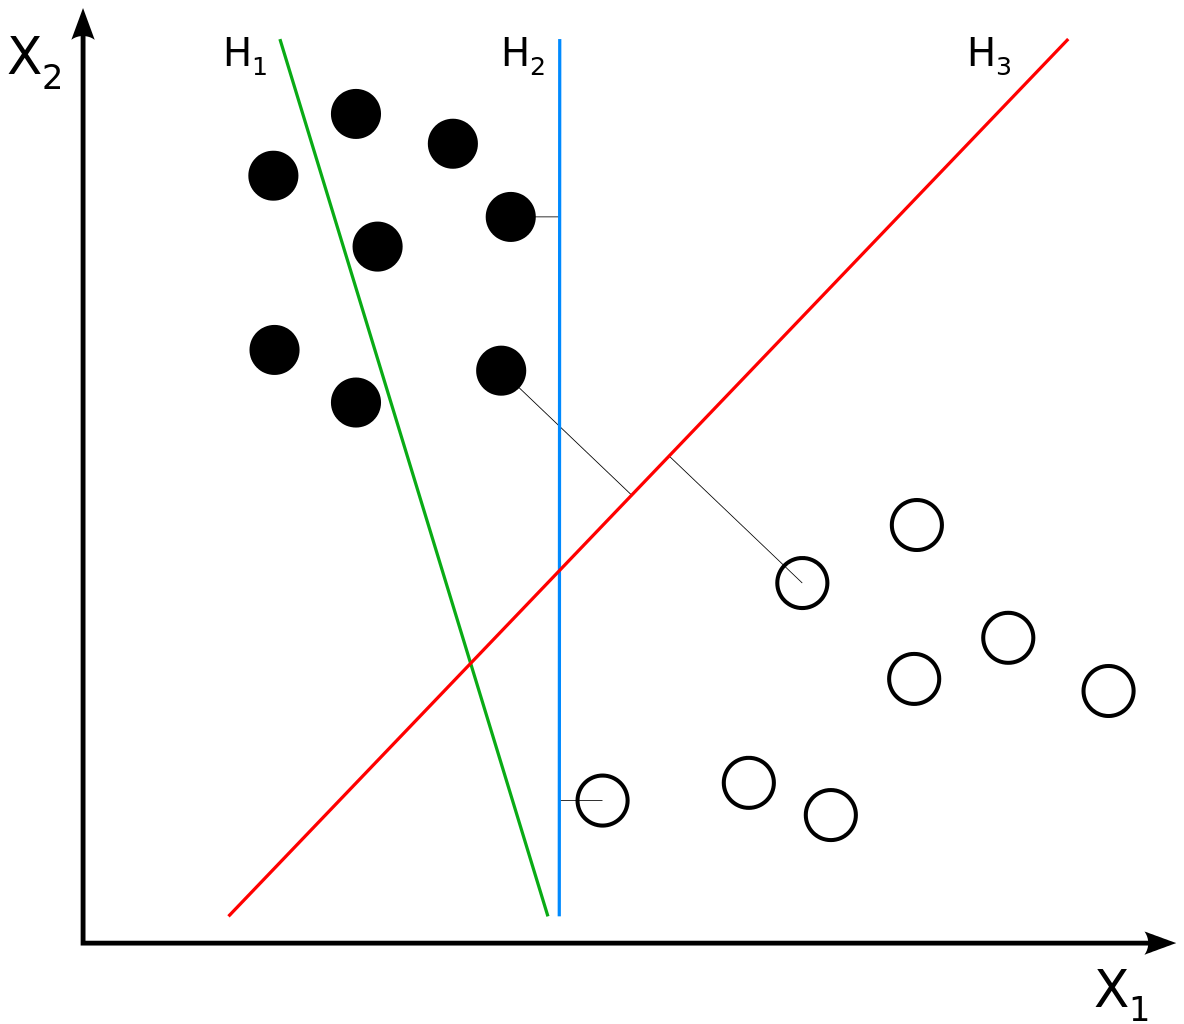
\includegraphics[width=10cm]{figures/1174080/2/1.png}}
\caption{Binary Classification}
\label{labelgambar}
\end{figure}

\item Tes Medis 

untuk menentukan apakah pasien memiliki penyakit tertentu atau tidak - properti klasifikasi adalah keberadaan penyakit.

\item Metode Uji ”lulus atau gagal” atau "kontrol kualitas di pabrik"

yaitu memutuskan apakah suatu spesifikasi telah atau belum terpenuhi - klasifikasi Go/no go.

\item Pengambilan informasi

yaitu memutuskan apakah suatu halaman atau artikel harus dalam hasil pencarian atau tidak - properti klasifikasi adalah relevansi artikel, atau kegunaannya bagi pengguna.
\end{enumerate}

\subsubsection{Supervised Learning , Unsupervised Learning dan Clusterring dengan ilustrasi gambar }

\begin{enumerate}
\item Supervised Learning

Supervised Learning dalam bahasa indonesia adalah pembelajaran yang ada supervisornya. Maksud disini ada supervisornya adalah label di tiap data nya. Label maksudnya adalah tag dari data yang ditambahkan dalam machine learning model. Contohnya gambar kucing di tag “kucing” di tiap masing masing image kucing dan gambar anjing di tag “anjing” di tiap masing gambar anjing. Machine learning kategori dapat berupa clasification (“anjing”, “kucing”, “beruang”, dsb) dan regression ( berat badan, tinggi badan dsb). Supervised learning banyak digunakan dalam memprediksi pola dimana pola tersebut sudah ada contoh data yang lengkap, jadi pola yang terbentuk adalah hasil pembelajaran data lengkap tersebut. Tentunya jika kita memasukan data baru, setelah kita melakukan ETL (Extract Transform Load) maka kita mendapat info feature feature dari sample baru tersebut. Kemudian dari feature feature tersebut di compare dengan pattern clasification dari model yang didapat dari labeled data. Setiap label akan dicompare sampai selesai, dan yang memiliki percentage lebih banyak akan diambil sebagai prediksi akhir.
\begin{figure}[H]
\centerline{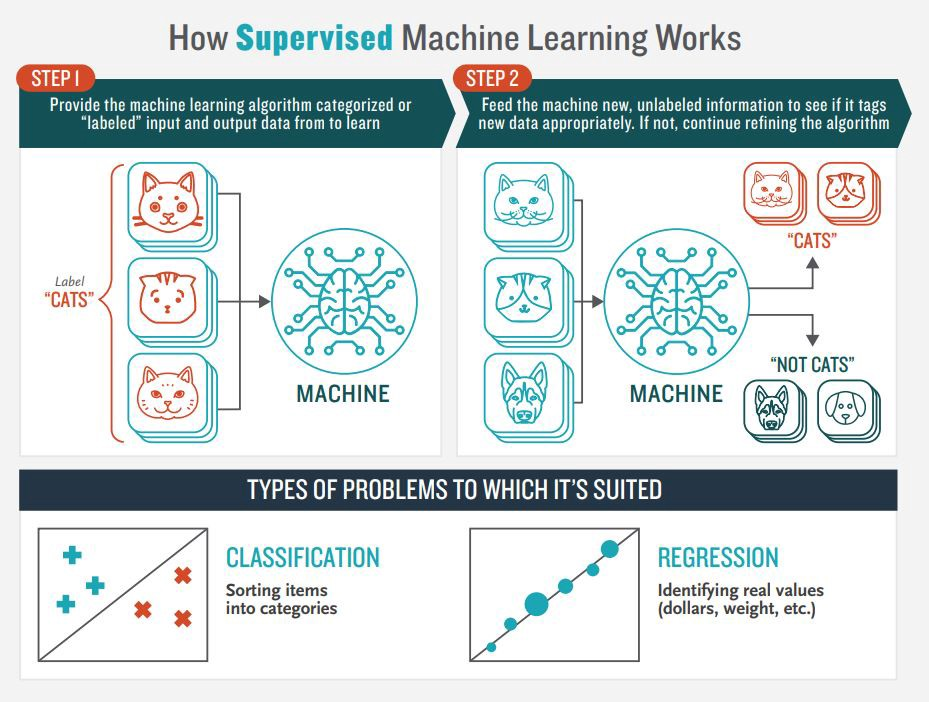
\includegraphics[width=10cm]{figures/1174080/2/2.jpeg}}
\caption{Supervised Learning}
\label{labelgambar}
\end{figure}

\item Unsupervised Learning

Unsupervised learning memiliki keunggulan daari unsupervised learning. Jika unsupervised learning memiliki label sebagai dasar prediksi baik serta membuat clasification dan regression algorithm memungkinkan. Tetapi dalam realitanya, data real itu banyak yang tidak memiliki label. Label kebanyakan jika data sudah masuk ke ERP apapun bentuk ERPnya dan bagaimana kalo datanya berupa natural input seperti suara, gambar, dan video. Unsupervised learning tidak menggunakan label dalam memprediksi target feautures / variable. Melainkan menggunakan ke samaan dari attribut attribut yang dimiliki. Jika attribut dan sifat sifat dari data data feature yang diekstrak memiliki kemirip miripan, maka akan dikelompok kelompokan (clustering). Sehingga hal ini akan menimbulkan kelompok kelompok (cluster). Jumlah cluster bisa unlimited. Dari kelompok kelompok itu model melabelkan, dan jika data baru mau di prediksi, maka akan dicocok kan dengan kelompok yang mirip mirip featurenya.
\begin{figure}[H]
\centerline{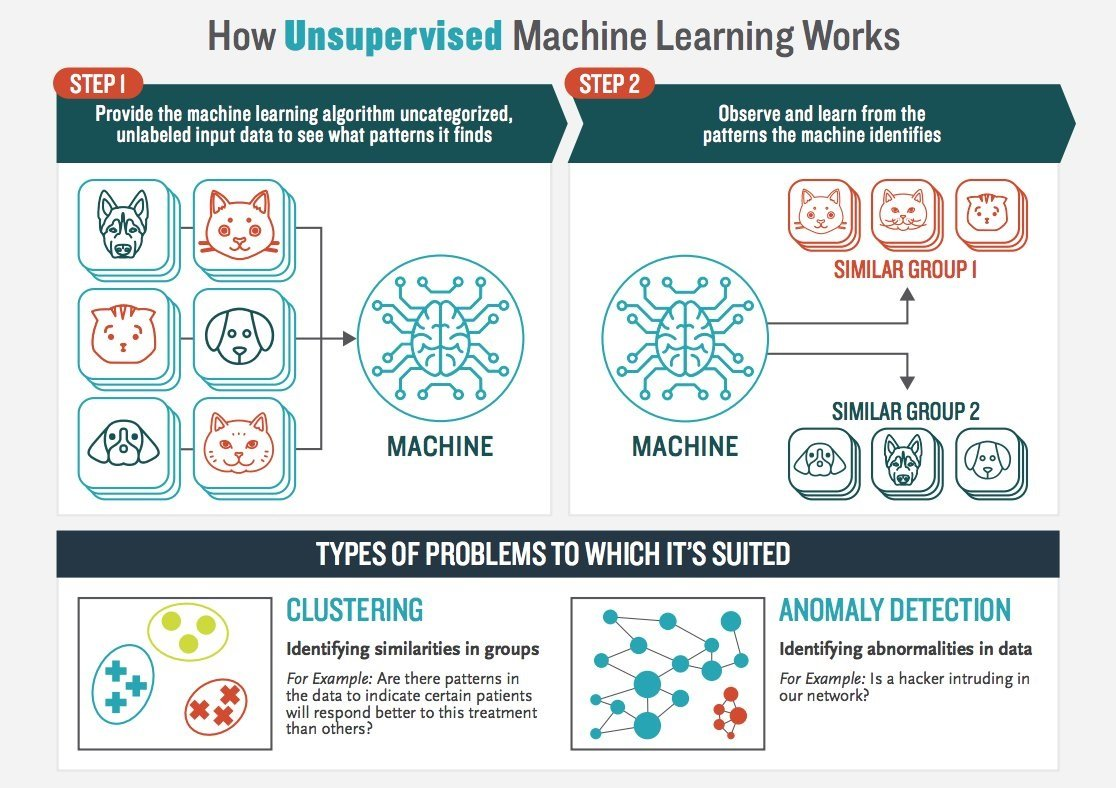
\includegraphics[width=10cm]{figures/1174080/2/3.jpg}}
\caption{Unsupervised Learning}
\label{labelgambar}
\end{figure}

\item Clusterring

Clustering atau klasterisasi adalah metode pengelompokan data. Menurut Tan, 2006 clustering adalah sebuah proses untuk mengelompokan data ke dalam beberapa cluster atau kelompok sehingga data dalam satu cluster memiliki tingkat kemiripan yang maksimum dan data antar cluster memiliki kemiripan yang minimum.
\begin{figure}[H]
\centerline{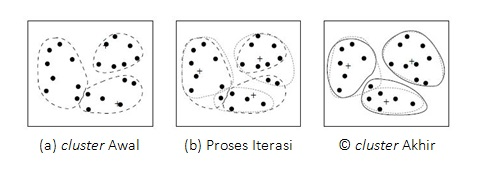
\includegraphics[width=10cm]{figures/1174080/2/4.jpg}}
\caption{Clusterring}
\label{labelgambar}
\end{figure}
\end{enumerate}

\subsubsection{Evaluasi dan Akurasi}

Evaluasi adalah tentang bagaimana kita dapat mengevaluasi seberapa baik model bekerja dengan mengukur tingkat akurasinya. Dan akurasi akan didefinisikan sebagai persentase kasus yang diklasifikasikan dengan benar. Kita dapat menganalisis kesalahan yang dibuat oleh model,atau tingkat kebingungannya, menggunakan matriks kebingungan(confusion matrix). Matriks kebingungan mengacu pada kebingungan dalam model,tetapi matriks kebingungan ini bisa menjadi sedikit sulit untuk dipahami ketika mereka menjadi sangat besar.
\begin{figure}[H]
\centerline{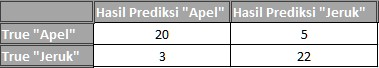
\includegraphics[width=10cm]{figures/1174080/2/5.jpg}}
\caption{Evaluasi}
\label{labelgambar}
\end{figure}

\subsubsection{Cara Membuat Confusion Matrix}

Confusion Matrix merupakan metode untuk menghitung akurasi pada data mining atau Sistem Pendukung Keputusan. Untuk menggunakan Confusion Matrix, ada 4 istilah sebagai hasil proses dari klasifikasi. Diantaranya adalah:
\begin{itemize}
\item True Positive: Data positif yang terdeteksi memiliki hasil benar
\item False Positive: Data Positif yang terdeteksi memiliki hasil salah
\item True Negative: Data negatif yang terdeteksi memiliki hasil benar
\item False Negative: Data negatif yang terdeteksi memiliki hasil salah
\end{itemize}
\begin{figure}[H]
\centerline{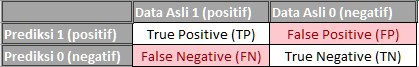
\includegraphics[width=10cm]{figures/1174080/2/6.jpg}}
\caption{Contoh Confusion Matrix}
\label{labelgambar}
\end{figure}

\subsubsection{Bagaimana Fold-cross validation}

Cross-validation (CV) adalah metode statistik yang dapat digunakan untuk mengevaluasi kinerja model atau algoritma dimana data dipisahkan menjadi dua subset yaitu data proses pembelajaran dan data validasi / evaluasi. Model atau algoritma dilatih oleh subset pembelajaran dan divalidasi oleh subset validasi. Selanjutnya pemilihan jenis CV dapat didasarkan pada ukuran dataset. Biasanya CV K-fold digunakan karena dapat mengurangi waktu komputasi dengan tetap menjaga keakuratan estimasi.

\begin{figure}[H]
\centerline{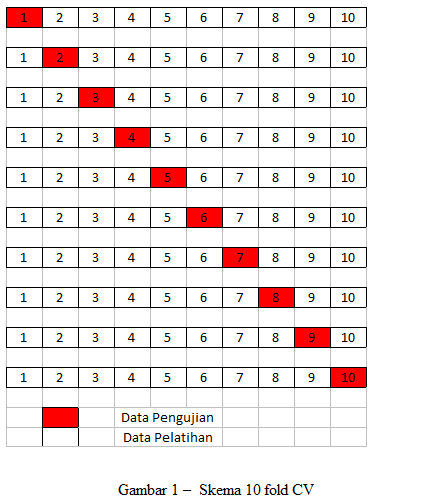
\includegraphics[width=10cm]{figures/1174080/2/7.png}}
\caption{Contoh Fold-Cross Validation}
\label{labelgambar}
\end{figure}
\begin{enumerate}
\item 10 fold CV adalah salah satu K fold CV yang direkomendasikan untuk pemilihan model terbaik karena cenderung memberikan estimasi akurasi yang kurang bias dibandingkan dengan CV biasa, leave-one-out CV dan bootstrap. Dalam 10 fold CV, data dibagi menjadi 10 fold berukuran kira-kira sama, sehingga kita memiliki 10 subset data untuk mengevaluasi kinerja model atau algoritma. Untuk masing-masing dari 10 subset data tersebut, CV akan menggunakan 9 fold untuk pelatihan dan 1 fold untuk pengujian seperti diilustrasikan pada Gambar diatas.
\end{enumerate}

\subsubsection{Decision Tree}

Decision Tree adalah sebuah struktur yang menentukan keputusan dan setiap konsekuensinya. Hasil dari setiap struktur biasanya menggunakan jawaban (True dan False) atau cabang lain yang akan menjadi pohon selanjutnya. Setiap keputusan diantaranya akan membandingkan kondisi yang diberikan kepada struktur untuk dibandingkan kondisi apa saja yang sudah didapat pada sistem tersebut.
\begin{figure}[H]
\centerline{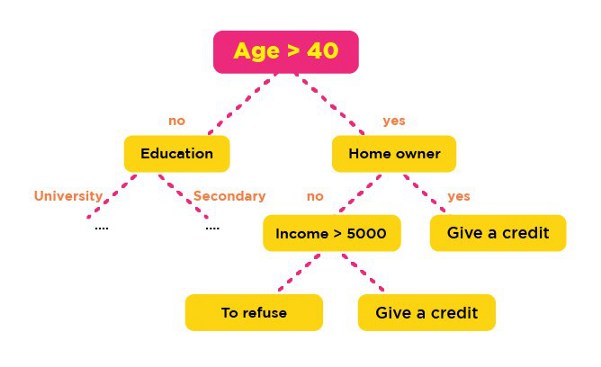
\includegraphics[width=10cm]{figures/1174080/2/8.png}}
\caption{Contoh Decision Tree}
\label{labelgambar}
\end{figure}

\subsubsection{Information Gain dan Entropi}
\begin{itemize}
\item Information Gain

Information Gain merupakan total data yang didapat dari data - data acak yang data tersebut akan digunakan untuk analisis data lainnya. Information Gain ini digunakan pada decision tree sebagai label setiap aksi - aksi yang perlu dinilai validasinya.
\begin{figure}[H]
\centerline{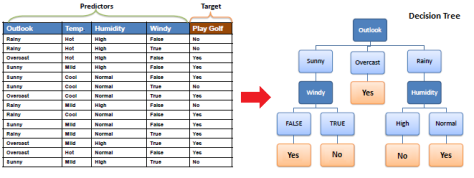
\includegraphics[width=10cm]{figures/1174080/2/9.png}}
\caption{Information Gain}
\label{labelgambar}
\end{figure}

\item Entropi

Entropi merupakan pengukuran sebuah data dan validnya data tersebut untuk dapat digunakan sebagai informasi yang akan dimasukkan ke Information Gain. Entropi menilai sebuah obyek berdasarkan kebutuhan di dunia nyata dan pengaruh pada sistem yang akan digunakan.
\begin{figure}[H]
\centerline{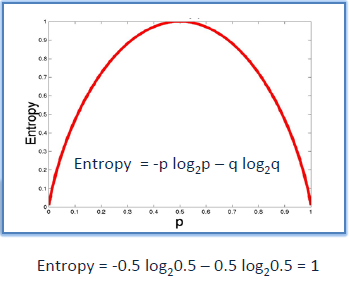
\includegraphics[width=10cm]{figures/1174080/2/10.png}}
\caption{Entropi}
\label{labelgambar}
\end{figure}
\end{itemize}


\subsection{Praktek}
Tugas anda adalah, dataset ganti menggunakan student-mat.csv dan mengganti semua nama variabel dari kode di bawah ini dengan nama-nama makanan (NPM mod 3=0), kota (NPM mod 3=1), buah (NPM mod 3=2)
\lstinputlisting[firstline=8, lastline=9]{src/1174080/2/1174080.py} 

\subsubsection{Nomor 1}
\hfill\\
\lstinputlisting[firstline=12, lastline=14]{src/1174080/2/1174080.py}
\begin{figure}[H]
\centerline{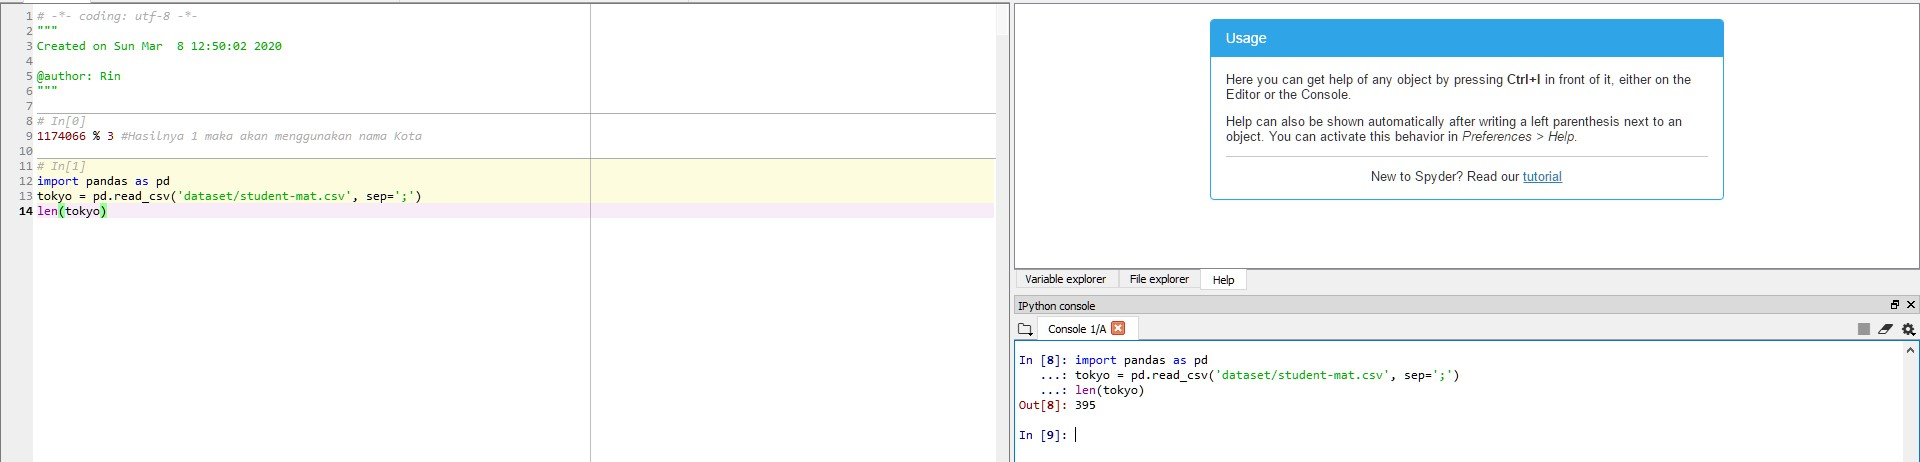
\includegraphics[width=10cm]{figures/1174080/2/11.jpg}}
\caption{Nomor 1}
\label{labelgambar}
\end{figure}

\subsubsection{Nomor 2}
\hfill\\
\lstinputlisting[firstline=16, lastline=20]{src/1174080/2/1174080.py}
\begin{figure}[H]
\centerline{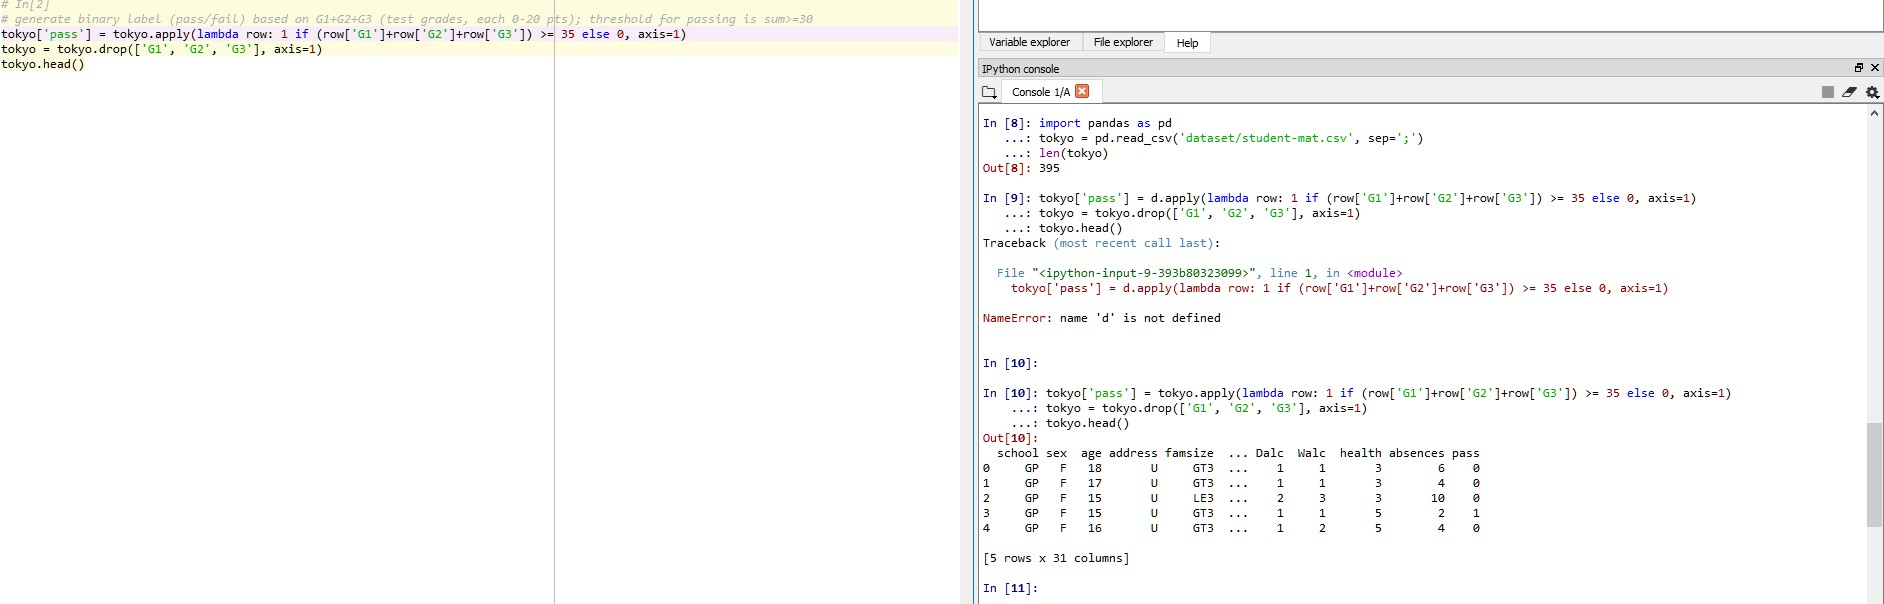
\includegraphics[width=10cm]{figures/1174080/2/12.jpg}}
\caption{Nomor 2}
\label{labelgambar}
\end{figure}

\subsubsection{Nomor 3}
\hfill\\
\lstinputlisting[firstline=22, lastline=27]{src/1174080/2/1174080.py}
\begin{figure}[H]
\centerline{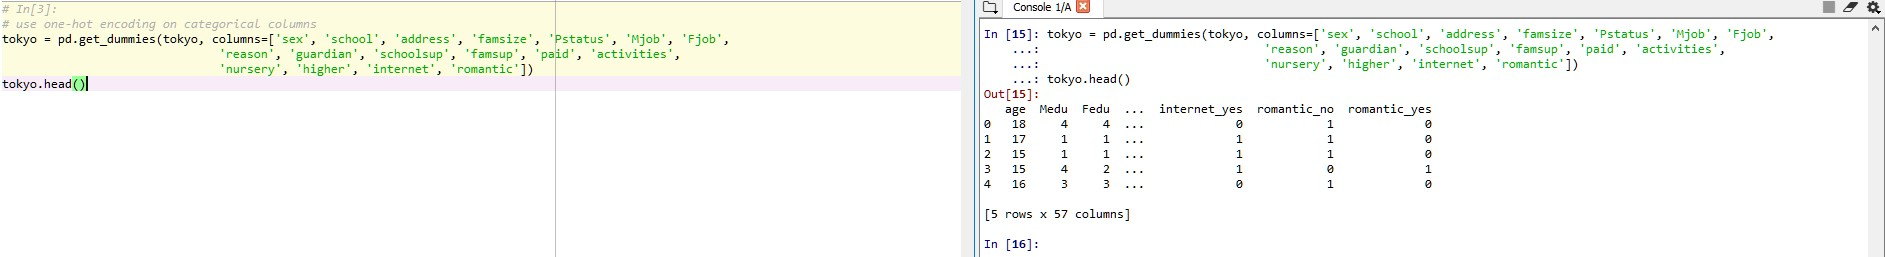
\includegraphics[width=10cm]{figures/1174080/2/13.jpg}}
\caption{Nomor 3}
\label{labelgambar}
\end{figure}

\subsubsection{Nomor 4}
\hfill\\
\lstinputlisting[firstline=29, lastline=47]{src/1174080/2/1174080.py}
\begin{figure}[H]
\centerline{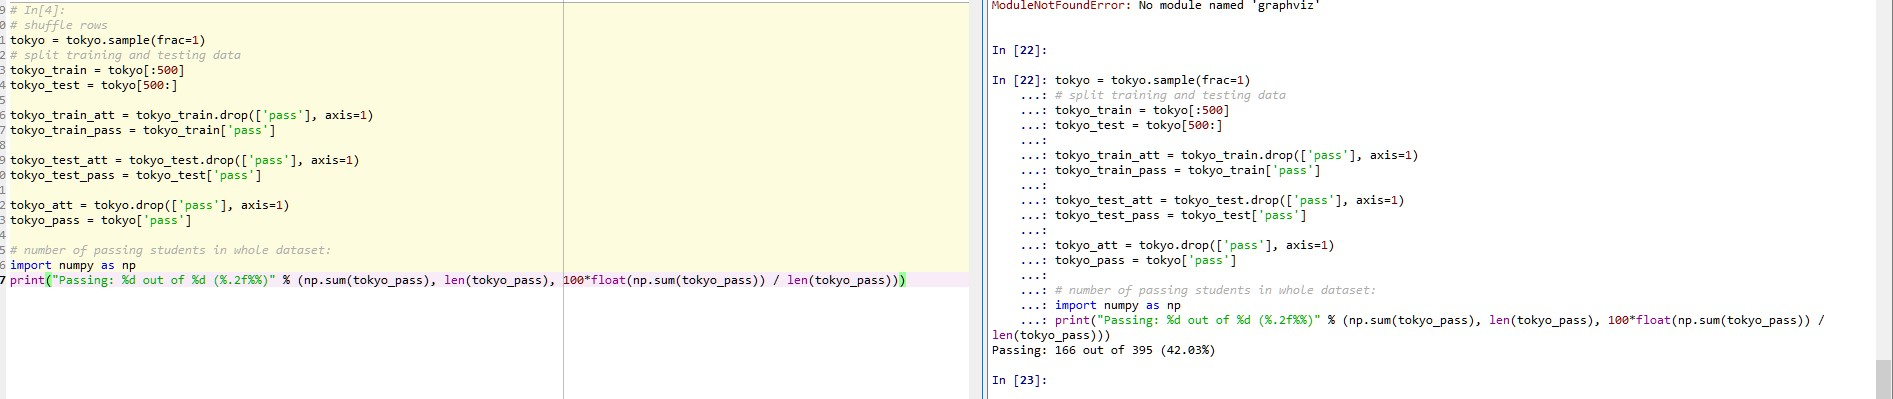
\includegraphics[width=10cm]{figures/1174080/2/14.jpg}}
\caption{Nomor 4}
\label{labelgambar}
\end{figure}

\subsubsection{Nomor 5}
\hfill\\
\lstinputlisting[firstline=49, lastline=53]{src/1174080/2/1174080.py}
\begin{figure}[H]
\centerline{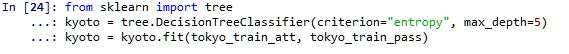
\includegraphics[width=10cm]{figures/1174080/2/15.jpg}}
\caption{Nomor 5}
\label{labelgambar}
\end{figure}

\subsubsection{Nomor 6}
\hfill\\
\lstinputlisting[firstline=56, lastline=63]{src/1174080/2/1174080.py}
\begin{figure}[H]
\centerline{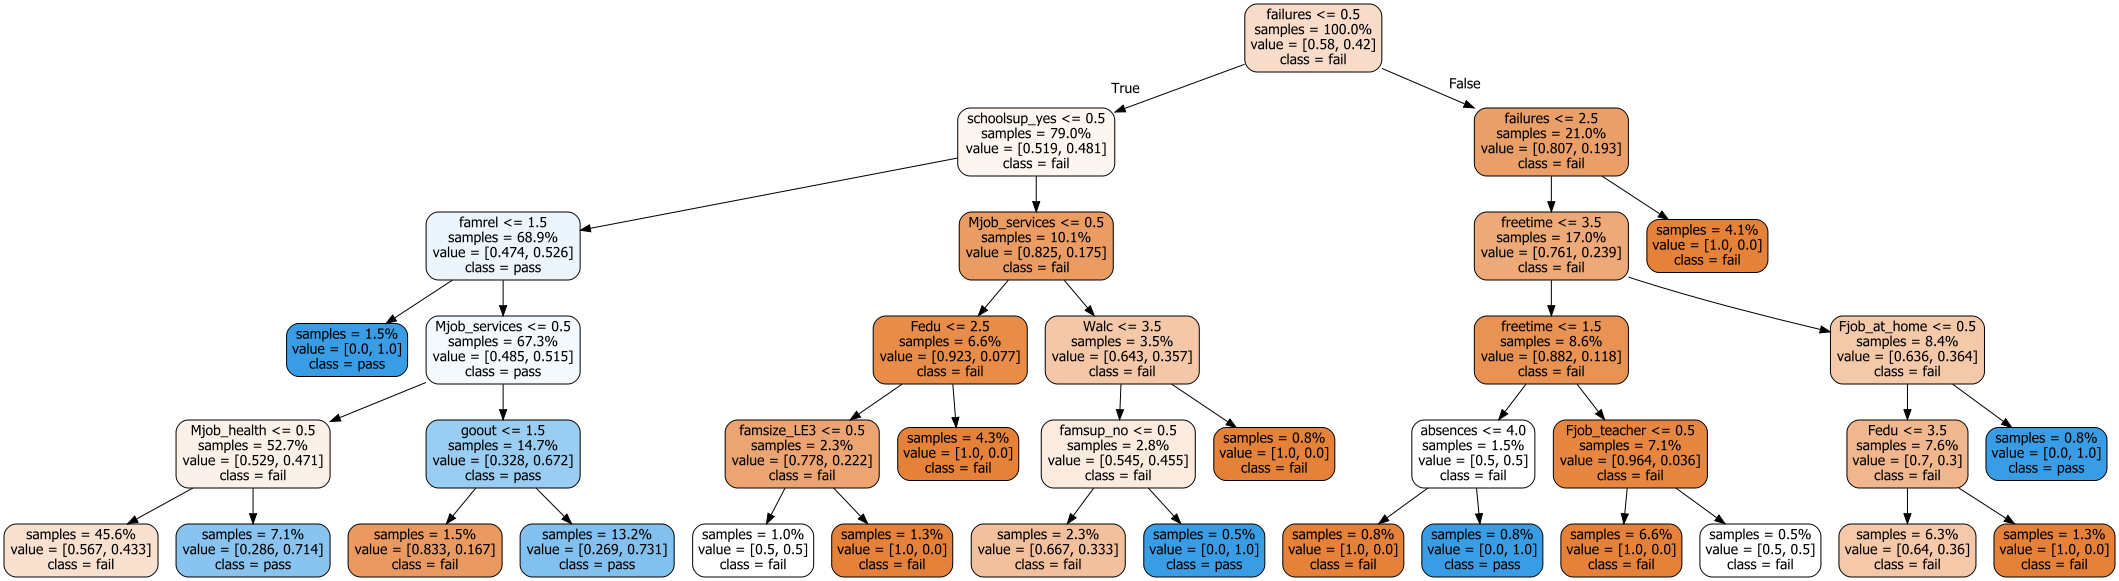
\includegraphics[width=10cm]{figures/1174080/2/16.png}}
\caption{Nomor 6}
\label{labelgambar}
\end{figure}

\subsubsection{Nomor 7}
\hfill\\
\lstinputlisting[firstline=66, lastline=70]{src/1174080/2/1174080.py}
\begin{figure}[H]
\centerline{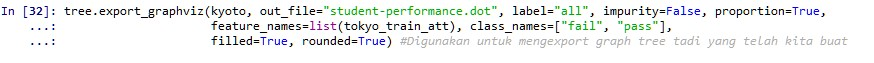
\includegraphics[width=10cm]{figures/1174080/2/17.jpg}}
\caption{Nomor 7}
\label{labelgambar}
\end{figure}

\subsubsection{Nomor 8}
\hfill\\
\lstinputlisting[firstline=73, lastline=74]{src/1174080/2/1174080.py}
\begin{figure}[H]
\centerline{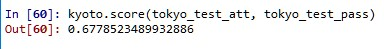
\includegraphics[width=10cm]{figures/1174080/2/18.jpg}}
\caption{Nomor 8}
\label{labelgambar}
\end{figure}

\subsubsection{Nomor 9}
\hfill\\
\lstinputlisting[firstline=77, lastline=81]{src/1174080/2/1174080.py}
\begin{figure}[H]
\centerline{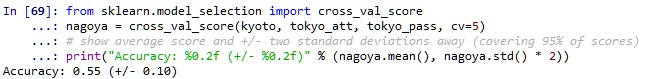
\includegraphics[width=10cm]{figures/1174080/2/19.jpg}}
\caption{Nomor 9}
\label{labelgambar}
\end{figure}

\subsubsection{Nomor 10}
\hfill\\
\lstinputlisting[firstline=84, lastline=88]{src/1174080/2/1174080.py}
\begin{figure}[H]
\centerline{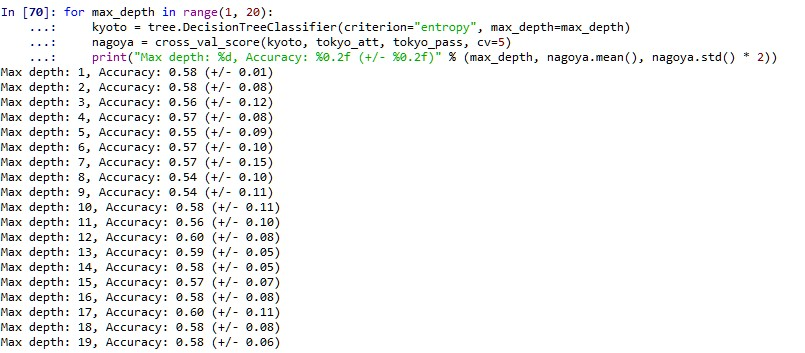
\includegraphics[width=10cm]{figures/1174080/2/20.jpg}}
\caption{Nomor 10}
\label{labelgambar}
\end{figure}

\subsubsection{Nomor 11}
\hfill\\
\lstinputlisting[firstline=91, lastline=102]{src/1174080/2/1174080.py}
\begin{figure}[H]
\centerline{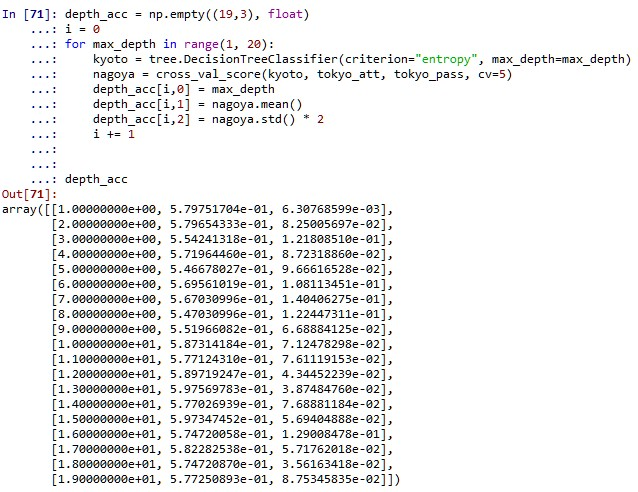
\includegraphics[width=10cm]{figures/1174080/2/21.jpg}}
\caption{Nomor 11}
\label{labelgambar}
\end{figure}

\subsubsection{Nomor 12}
\hfill\\
\lstinputlisting[firstline=105, lastline=109]{src/1174080/2/1174080.py}
\begin{figure}[H]
\centerline{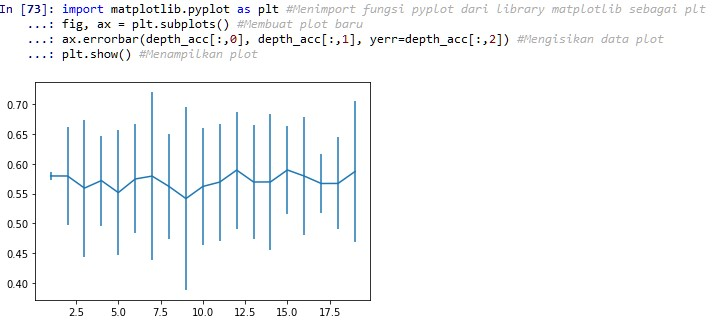
\includegraphics[width=10cm]{figures/1174080/2/22.jpg}}
\caption{Nomor 12}
\label{labelgambar}
\end{figure}

\subsection{Penanganan Error}
\subsubsection{Error}
\hfill\\
\begin{enumerate}
\item ModuleNotFoundError

\begin{figure}[H]
\centerline{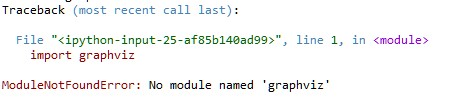
\includegraphics[width=10cm]{figures/1174080/2/error.jpg}}
\caption{ModuleNotFoundError}
\label{labelgambar}
\end{figure}
\end{enumerate}

\subsubsection{Solusi}
\begin{enumerate}
\item Intall library Graphviz dengan cara download graphviz di google

setelah instalasi buka anaconda prompt sebagai admin lalu mengetikkan
\begin{lstlisting}
conda install graphviz
\end{lstlisting} 
\end{enumerate}

\subsection{Bukti Tidak Plagiat}
\hfill\\
\begin{figure}[H]
\centerline{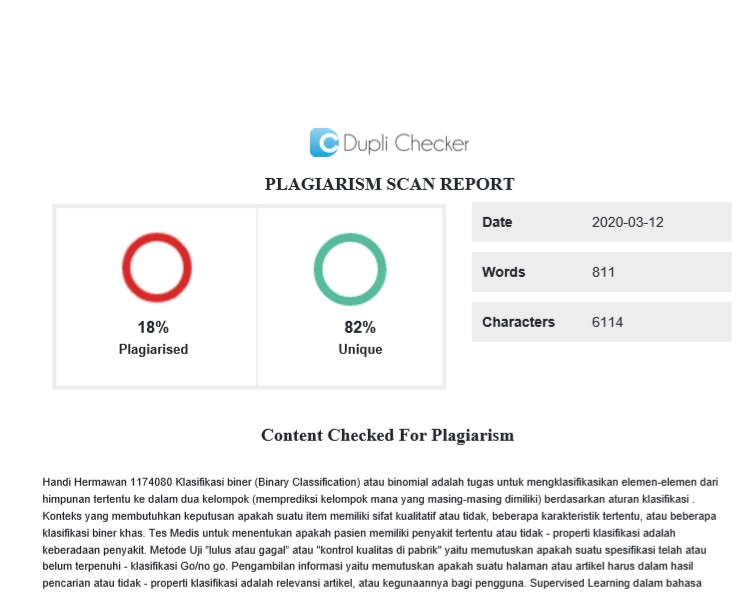
\includegraphics[width=10cm]{figures/1174080/2/plagiat.jpg}}
\caption{Bukti Tidak Plagiat}
\label{labelgambar}
\end{figure}

\subsection{Link Youtube:}
https://youtu.be/QL05oLFErFk
